
\documentclass[12pt,crop,tikz]{standalone}
\providecommand{\rootdir}{..}
\usetikzlibrary{positioning}
\usetikzlibrary{calc}
\usetikzlibrary{arrows}
\tikzstyle{arrow} = [thick,->,>=stealth]


% The Tableau20 colours
\definecolor{TabLightOrange}{RGB}{255,187,120}
\definecolor{TabOrange}{RGB}{255,127,14}
\definecolor{TabLightBlue}{RGB}{174,199,232}
\definecolor{TabBlue}{RGB}{31,119,180}
\definecolor{TabGreen}{RGB}{44,160,44}
\definecolor{TabLightGreen}{RGB}{152,223,138}
\definecolor{TabSalmon}{RGB}{255,152,150}
\definecolor{TabRed}{RGB}{214,39,40}
\definecolor{TabPurple}{RGB}{148,103,189}
\definecolor{TabLightPurple}{RGB}{197,176,213}
\definecolor{TabLightPink}{RGB}{247,182,210}
\definecolor{TabPink}{RGB}{227,119,194}
\definecolor{TabLightBrown}{RGB}{196,156,148}
\definecolor{TabBrown}{RGB}{140,86,75}
\definecolor{TabGray}{RGB}{127,127,127}
\definecolor{TabOlive}{RGB}{188,189,34}
\definecolor{TabLightOlive}{RGB}{219,219,141}
\definecolor{TabLightGray}{RGB}{199,199,199}
\definecolor{LightCyan}{RGB}{158,218,229}
\definecolor{TabCyan}{RGB}{23,190,207}

\begin{document}
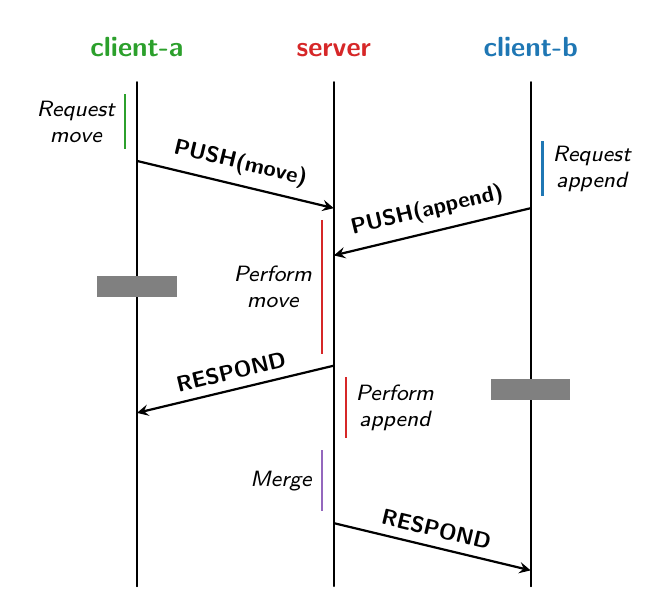
\begin{tikzpicture}
  [ every node/.style={font=\footnotesize\sffamily}
  , action/.style={-, draw=black!40}
  , timeline/.style={-, thick, line cap=round}
  , timeline-label/.style={font=\normalsize\sffamily\bfseries}
  , message-label/.style={midway, sloped, above,font=\footnotesize\sffamily\bfseries}
  , action-label/.style={midway, align=center, color=black, font=\footnotesize\sffamily\itshape}
  , blocked/.style={midway, fill=white, gray, outer sep=0pt, inner sep= 1pt}
  , arrow={->,>=stealth}
  ]

  \def\actionspace{0.15}
  \def\spacing{2.5}
  \def\height{6.4}
  \def\arrowdy{0.6}
  \def\labelspace{0.2cm}
  \def\worklength{1.6}
  
  \coordinate (clienta-origin) at (0, 0);
  \coordinate (server-origin) at ($ (clienta-origin) + (\spacing, 0) $);
  \coordinate (clientb-origin) at ($ (server-origin) + (\spacing, 0) $);

  \coordinate(request1-start) at ($ (clienta-origin) $);
  \coordinate(request1-end) at ($ (request1-start) + (0, -1) $);

  \coordinate(request2-start) at ($ (clientb-origin) + (0, -0.6) $);
  \coordinate(request2-end) at ($ (request2-start) + (0, -1) $);

  \coordinate (perform1-start) at ($ (request1-end) + (\spacing, -\arrowdy)$);
  
  \coordinate (perform1-end) at ($ (perform1-start) + (0, -2)$);
  \coordinate (respond1-end) at ($ (perform1-end) + (-\spacing, -\arrowdy) $);

  \coordinate (perform2-end) at ($ (perform1-end) + (0, -1) $);
  \coordinate (merge-end) at ($ (perform2-end) + (0, -1) $);

  \coordinate (respond2-end) at ($ (merge-end) + (\spacing, -\arrowdy) $);
  
  \pause

  \node[timeline-label, above = 0.2cm of clienta-origin] (clienta-label) {\bfseries\textcolor{TabGreen}{client-a}};
  \node[timeline-label, above = 0.2cm of server-origin] (server-label) {\bfseries\textcolor{TabRed}{server}};
  \node[timeline-label, above = 0.2cm of clientb-origin] (clientb-label) {\bfseries\textcolor{TabBlue}{client-b}};

  \coordinate (clienta-end) at ($ (clienta-origin) + (0, -\height) $);
  \coordinate (clientb-end) at ($ (clientb-origin) + (0, -\height) $);

  % Draw initial timelines
  \draw[timeline] (clienta-origin) -- (request1-end);
  \draw[timeline] (server-origin) -- +(0, -\height);
  \draw[timeline] (clientb-origin) -- (request2-end);

  % Client A timeline
  \onslide<2-3>{ 
    \draw[timeline] (request1-end) -- (clienta-end);
  }

  \onslide<4-7>{
    \draw[-, dashed] (request1-end) -- node[blocked] {blocked} (respond1-end) -- (clienta-end);
  }

  \onslide<8->{
    \draw[-, dashed] (request1-end) -- node[blocked] {blocked} (respond1-end); % shorten the dotted line
    \draw[-, dashed] (request1-end) -- node[blocked] {blocked} (respond1-end);
    \draw[timeline] (respond1-end) -- (clienta-end);
  }

  % Client B timeline
  \onslide<2-5>{
    \draw[timeline] (request2-end) -- (clientb-end);
  }

  \onslide<6-10>{
    \draw[-, dashed] (request2-end) -- node[blocked] {blocked} (respond2-end) -- (clientb-end);
  }

  \onslide<11->{
    \draw[-, dashed] (request2-end) -- node[blocked] {blocked} (respond2-end); % shorten the dotted line
    \draw[timeline] (respond2-end) -- (clientb-end);
  }
  
  \pause

  % Client A requests a move
  \draw[action, color=TabGreen] ($ (request1-start) + (-\actionspace, -\actionspace) $) -- node[action-label, left] {Request\\move} ($ (request1-end) + (-\actionspace, \actionspace) $);
  \pause

  % Client A pushes to the server
  \draw[->] ($ (request1-end)  $) -- (perform1-start) node[message-label] {\footnotesize\textbf{PUSH(move)}};
  \pause

  \draw[action, color=TabBlue] ($ (request2-start) + (\actionspace, -\actionspace) $) -- node[action-label, right] {Request\\append} ($ (request2-end) + (\actionspace, \actionspace) $);
  \pause
  
  \draw[->] ($ (request2-end)  $) -- +(-\spacing, -\arrowdy) node[message-label] {\footnotesize\textbf{PUSH(append)}};
  \pause

  \draw[action, color=TabRed] ($ (perform1-start) + (-\actionspace, -\actionspace) $) -- node[action-label, left] {Perform\\move} ($ (perform1-end) + (-\actionspace, \actionspace) $);
  \pause

  \draw[->] (perform1-end) -- (respond1-end) node[message-label] {\footnotesize\textbf{RESPOND}};
  \pause

  \draw[action, color=TabRed] ($ (perform1-end) + (\actionspace, -\actionspace) $) -- node[action-label, right] {Perform\\append} ($ (perform2-end) + (\actionspace, 0.5*\actionspace) $);
  \pause

  \draw[action, color=TabPurple] ($ (perform2-end) + (-\actionspace, -0.5*\actionspace) $) -- node[action-label, left] {Merge} ($ (merge-end) + (-\actionspace, \actionspace) $);
  \pause

  \draw[->] (merge-end) -- (respond2-end) node[message-label] {\footnotesize\textbf{RESPOND}};

\end{tikzpicture}
\end{document}